%!TEX root = ../USthesis_Masters.tex
\chapter{System Design}
\label{chp:System Design}


%%%%%%%%%%%%%%%%%%%%%%%%%%%%%%%%%%%%%%%%%%%%%%%%%%%%%%%%%%%%%%%%%%%%%%%
\section{Framework}

In this project we test the viability of a payment framework on a mobile social media platform. The framework will consist of several independant but connected pieces:

\begin{itemize}
	\item REST API for payments
	\item Wallet Application
	\item Bitcoin Interface
	\item Use-case Application
\end{itemize}

A summary of what is required from the system can be seen in figure \ref{fig:summary_framework}.

\begin{figure}
  \centering
    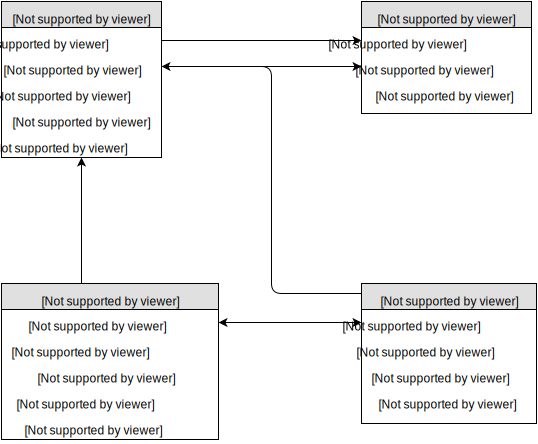
\includegraphics[width=0.7\textwidth]{figs/Summary.pdf}
   \caption{Summary of Framework} 
   \label{fig:summary_framework}
\end{figure}

\subsection{REST API for payment management}

A REST (Representational State Transfer) API \cite{Oracle.com} was chosen for the main interface for developers to use Bitcoin without running a Bitcoin node or having experience with Bitcoin. REST was chosen because it is a commonly used architecture, it is easy to use and understand and it does not constrain the user's choice of programming langauge or environment. 

The purpose of the REST API is to let developers make payment requests and check if a payment has been made, without dealing with the low-level Bitcoin transactions directly. Thus, our system should generate a new Bitcoin address on request. 

% We also require the developer to check wether a payment has been successfully made.
Our requirements from the REST API are:

\begin{itemize}
	\item New Bitcoin address for each payment
	\item Verify payment
	\item Check total balance of developer
	\item Witdraw available Bitcoin of developer
\end{itemize}

\subsubsection{The concept of the Bitcoin payment}

This is a high-level explanation of how to receive verifyable payments with Bitcoin. With Bitcoin, unlike a traditional bank account, you don't have a single ``account'' where people can make payments to and you can verify that the payment came from them. With Bitcoin it is trivially easy to make a new Bitcoin address, and it can be generated without being connected to the Internet or the Bitcoin network.

Since the entire Bitcoin blockchain is public, a single address is not sufficient to receive multiple payments. With a single address, it is not easy to verify that a spesific person has made a payment, since there may be several payments of the same amount happening in short succession.

The sollution to the problem is generating a new address for every payment, and requesting that the user make the payment to that address. Since the newly generated address is not yet present on the blockchain, when a payment to that address of the requested amount occurs, we can be certain that the person in question made the payment. When the payment is complete, the Bitcoin in that address can be transferred to a central address, and the original address can be discarded.

From our requirements for the REST API, we clearly require (at least) the following methods:

\begin{itemize}
	\item A payment method
	\item A balance method
	\item A payout method
\end{itemize}

\subsubsection{The /payment method}
\label{sct:payment}

The /payment method is the core of the REST API. It is used to make a payment request with a specified amount of Bitcoin and a description of the transaction. The /payment method returns a Bitcoin public address and a payment ID. 

The user can then pay to the Bitcoin address using any standard Bitcoin payment method, or can pay directly from the Bitcoin wallet that will run on WeChat and will be connected to the payment infrastructure.

\subsubsection{/payment/\{PUBLIC\_ADDRESS\} and /payment/\{ID\}}

These two methods are conceptually the same, but they take in two different arguments. The one takes the Bitcoin address to be queried, and the other takes the payment ID. The method returns all the data about the transaction, including the status of the transaction. 

The main purpose of this method is to verify that a transaction has been completed by the user. It can also be used to give the payment details to to user again.

\subsubsection{/balance}

The /balance method gives the developer the balance of all the available Bitcoin from all the received transactions. The method also returns a flag that says if there is enough Bitcoin to make a payout.

\subsubsection{/payout}

The /payout method is used by the developer to transfer all of the available Bitcoin to a specified Bitcoin address.

\subsection{Wallet Application}

The Wallet Application is a Bitcoin wallet implemented on the WeChat platform. The WeChat platform uses a simple message-answer structure. A user sends a message in the Wallet Application. The message is then sent to WeChat that sends it to a third party server controlled by the developer. The server then sends a reply to WeChat that is then forwarded to the user. 

In this manner, a fully functional Bitcoin wallet is realised. The third party server stores the private keys and processes the Bitcoin transactions on commands from the user.

The advantage of using the WeChat platform is the security built in to the platform, as well as an existing userbase. 

The Wallet Application will be directly connected to the back-end of the REST API. Thus, payment requests will be referable directly from the Wallet Application without needing to reference the Bitcoin Address. It will be able to reference the request using the payment ID mentioned in \ref{sct:payment}

\subsection{Bitcoin Interface}
\label{sct:bitcoin_interface}

To connect to the Bitcoin peer-to-peer network, a Bitcoin client is needed. The standard way of doing this is running the Bitcoin open source software on a server. This is very network and processor intensive. For development and testing, it will be quite expensive to run the Bitcoin software. Thus, an alternative is required for interfacing with the Bitcoin network. Fortunately, there are services that provide access to most of the Bitcoin operations using their API's. 

We require the following from such a service:

\begin{itemize}
	\item Get the balance from an address,
	\item Get unspent outputs from an address,
	\item Post a signed Bitcoin transaction to the network,
	\item It must be able to use the Testnet
\end{itemize}

The details of the chosen service is covered in chapter \ref{chp:Detail Design}.
% After considering several options, a service called chain.com was chosen. Chain.com is a free service that satisfies all the requirements. It is perfect to use this service as a proof of concept, but in practice one would rather run a full Bitcoin node to minimize reliance on third-party services.

\subsection{Use-case Application}

To use the payment framework, a Gamebook application is created to read Choose Your Own Adventure style books on the WeChat platform. User-created books can be sold by using the Bitcoin payment framework and the author can potentially earn Bitcoin.

For each sale, the Gamebook application creates a payment request using the REST API. The user can then pay using the Wallet Application or any Bitcoin payment mechanism. The Gamebook application can the query the API to confirm that the payment is received. 